\documentclass[hidelinks,12pt]{report}
\usepackage[utf8]{inputenc}
\usepackage{float}

\usepackage[margin=1.2in]{geometry}
\usepackage[T1]{fontenc}
\usepackage{graphicx}
\usepackage{pdfpages}
\usepackage{mathtools}
\usepackage{hyperref}
\usepackage{mathtools, bm}
\usepackage{amssymb, bm}
\usepackage{indentfirst}
\graphicspath{ {images/} }
%indent
\setlength{\parindent}{1em}
\setlength{\parskip}{1em}
%figures at the begining of page
\makeatletter
\setlength{\@fptop}{0pt}
\makeatother
%for tables
\newcommand{\bigcell}[2]{\begin{tabular}{@{}#1@{}}#2\end{tabular}}

\begin{document}
\begin{center}
\begin{large}
\textbf{Acknowledgment} 
\end{large}\\~\\
\end{center}
\par This project would have not been possible without the collaboration between the CNSMDP  (\textit{"Conservatoire National Supérieur de Musique et de Danse de Paris"}) and the laboratory of IRCCYN (\textit{"Institut de Recherche en Communications et Cybernétique de NantesWebsiteDirections
"}). I would like to thank especially Dr. Mathieu Lagrange who has put his trust in me on completing this project for his guidance all along my internship and his suggestions that helped me achieve the anticipated results.\\ I would also like to thank, soon to be doctor vincent Lonstanlen, for his guidance on how to use the matlab box Scatnet, and his suggestions during the progress of my internship.
\thispagestyle{empty}
\newpage
\tableofcontents
\thispagestyle{empty}
\newpage
\clearpage
\thispagestyle{empty}
\newpage
\listoffigures
\thispagestyle{empty}
\newpage
\clearpage
\setcounter{page}{1}
\noindent




\chapter{Introduction}
\section{CNSMDP and Project TICEL.}
The CNSMDP  (\textit{"Conservatoire National Supérieur de Musique et de Danse de Paris"}) offers a high level training in the domain of music,dance and sound technologies. Placed under the tutelage of the French Ministry of Culture and Communication, the conservatory offers to its 1300 students a cutting edge study programmes. Also, to keep up with the new technologies and help in its advancement, a lot of projects are launched to benefit from the digital advancement in the musical and dance domains. \\
The project TICEL (\textit{"Traité instrumental collaboratif en ligne"}) falls directly in that perspective. It was launched in collaboration between the CNSMDP, "\textit{'Ecole normale supérieure de Paris}" and \textit{"Ecole centrale de Nantes"}. The project was thus supervised by Dr. Mathieu Lagrange at the laboratory of IRCCYN (\textit{"Institut de Recherche en Communications et Cybernétique de Nantes"}) in the city of Nantes. I was asked as part of my final year project to conduct an internship on the project. \par
The purpose of the internship is to study the sounds played by different instruments with different playing techniques. The music samples will thus be represented in a space of descriptors that enables the  discrimination between two instruments and their relative playing techniques. This discrimination is done by finding a space where an euclidean distance is maximum for inter-class observations and minimum for intra-class observations. The precision of the space will be evaluated using two ranking metrics : the mean average precision (MAP) and the precision at k (P@k). The study was done on the SOL database that is presented in the next paragraph.  \\ 

\section{The SOL database.}
The SOL database is provided as part of the Orchids orchestration system by the team IRCAM. It contains 25119 audio files stored in the 24 bits / 44.1 kHz format. The sounds are played by 16 different instruments which can be subdivided into 32 different classes. There are 498 different combination of instrument with different playing techniques. The database contains three types of instruments varying from strings (Violin, Viola, ...), woodwind (Flute, Oboe...) and Brass (Trumpet, Trombone,...). The techniques of playing on each instruments vary from instrument to another and include techniques such as Aeolian, crescendo, flatterzunge... A full list of instruments and playing techniques is provided in \cite{SOL}.
Figure 2.1 shows the distribution of the SOL database along 6 octaves and one non acoustic class. The biggest part is octave 4 where all the instruments are represented in it (with different proportions).

\begin{figure}[t!]
  
  \centering
	    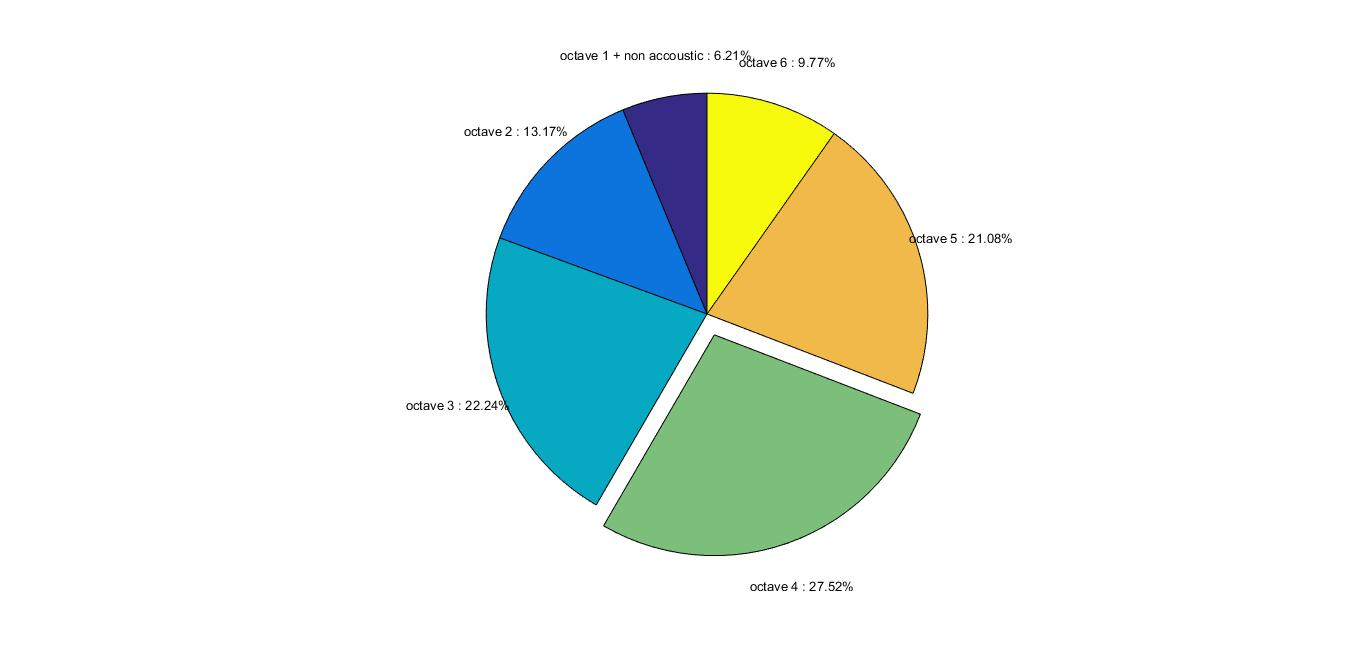
\includegraphics[width=1\textwidth]{byoctave}
    \caption{Musical octave study of sol database}
\end{figure}


\section{Human interpretation and timber.}

Before we start presenting the work done in this internship it will be interesting to look on how this discrimination is naturally done by human.\par
\begin{figure}[t!]
  
  \centering
	    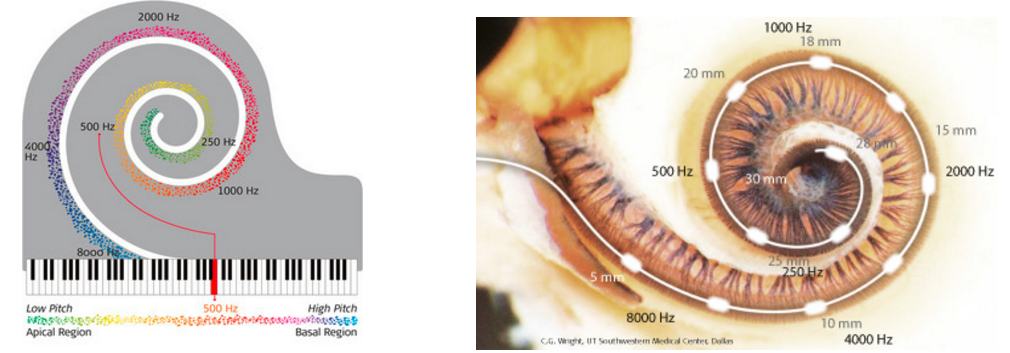
\includegraphics[width=1\textwidth]{cochlear}
    \caption{scheme of the cochlear taken from : http://www.medel.com/uk/show2/index/id/1361/title/Complete-Cochlear-Coverage/}
\end{figure}
\subsection{The mechanics of hearing.}
Our brain processes sounds by analyzing both the frequency components of those signals and the temporal change of amplitude. To better understand this phenomena, the figure 1 shows a scheme of the cochlear inside the ear. We can see on the right part of the picture, that the cochlear contains hair resonating  at different frequencies. Those small hair will trigger a nerve. this nerve will inform the brain on which frequencies is being heard by the ear. The brain will thus have three information to process, the frequencies, their relative loudness and the time they are being heard. Based on those three information the sound will be constructed, and we will be able to   
recognize the loudness, pitch and timbre of the sounds we are hearing. Other perception factors can help in recognizing the spacial coordinates   of that sound.

\subsection{The psychology of hearing.}

In our daily interaction with our environment, what is relevant is not what we perceive but how we interpret it.For example, hearing the sound of a train behind us is directly correlated with fear. Another example more relevant to our study, a french person hearing an arabic song will react to it differently from a native person. To fully understand how we interpret sound, the mechanical factors inside the ear are not enough. Just as all the other senses, a psychological aspect should be taken into account to build the hole picture of our interpretation of reality. This aspect can not be explained with equations, rather it is better understood with experiences or with functional study of the brain. In the last section of our internship we will be dealing with one similar problem of understanding the psychology of interpreting instrument sounds.\par 


I will be presenting in this report the study of similarity between different audio recordings coming from same and different instruments with different playing technique, and since timber by its most general definition is what allows us to experience, the same note played with the same loudness, in a different way for each instrument.\\ I will first start by talking about  timbre, then I will present the problem and its proposed solution. 



\section{What do we know about timbre ?}
Since the first explanation of sounds put by Helmholtz in 1863 \cite{H95}, the definition of timbre has changed, especially with the inability of modern day synthesizers to reproduce the same auditory experience of an instrument based on a primal definition of timbre. After a lot of studies done on the subject by physicists, biologists and musicians we have a clear definition of what timbre is not rather than what it really is. For instance, the American National Standard Institute ANSI in the American National Standard on Acoustical Terminology (\textit{ANSI S1.1-1994}) defines timbre as follows :
\begin{quote}
\textit{"Timbre is that attribute of auditory sensation in terms of which a listener can judge that two sounds similarly presented and having the same loudness and pitch are dissimilar." ANSI 1994}
\end{quote}
This definition clearly states that timbre is not related to the loudness, pitch or the duration of the tune being played (or spoken). This being said, There are still many factors that help us distinguish between two notes played with the same loudness, pitch and duration, those factors are considered as part of the structure of timbre. Some example of those factors:
\begin{itemize}
\item The difference in amplitude of the harmonics.
\item Change in harmonics during the attack.
\item The deviation of the harmonics from the perfect $n*f$ location where f is the fundamental note and n is an integer.
\item The vibrato of the note.
\item The sustain and the decay of the note. 
\end{itemize}
The notion of timbre is still an abstract one, thus it will be an obvious step to try to find another solution to solve the problem.
\section{Defining the problem.}
To try and achieve the best results, the project was divided into two parts. The first part is based on the true labeling of the data and the second part is based on a ground truth experiment conducted on 78 samples.
\subsection{True labeling problem.}
In the first section of the project, we studied the complete Sol database by dividing it into classes. We studied three type of classes :
\begin{enumerate}
\item classes of instruments.
\item classes of instruments with variation(with mute, without mute...).
\item classes of instruments with different playing techniques.
\end{enumerate}
In this part, the labeling is taken from the true nature of the instrument , and no human opinion affects the decision of the labeling. We are thus facing the problem of discriminating between instruments based on the physical aspect of the instruments. It should be noted that the difficulty of the problem increment with the number of classes. For example, twe have more different factors between two instruments than two instruments played in the same technique.\\ The anticipated end result is to find the space where the five nearest neighboors to each sample are from the same class.

\subsection{Ground truth labeling.}
In the second section of the project, a ground truth study was conducted and 32 different subjects gave labeling based on their interpretation of 78 samples taken from the complete database. This time the labeling is affected by the psychological way each person hear the sound. The similarity between two samples is not only based on the true nature of the sound but also on how each subject interpret the sound.\\ What we are searching to achieve in this section is that the five nearest samples are from the same class based on the average opinion of all the test subjects.

\section{How we adressed the problem}
In both cases, we have to identify the space in which we are trying to classify our data and proceed to proper feature extraction. We have two ways of looking at the feature extraction problem : perceptual or taxonomic \cite{P03}. The perceptual approach is motivated by the biological aspect of the problem, and it aims to explain how we hear the sound by finding a space where the descriptors axis explains the notion of timbre. We will not enter into details in this aspect, rather we will consider the taxonomic approach, in which the best feature space is the one that helps in getting the most discrimination between classes.\par
A state of the art study was done on the subject of features extraction for audio samples. Based on that study, I will be considering two space representation; the first one is the MFCC and the other is the scattering \cite{AM11}. In both cases we will try to get the highest precision based on the Mean-Average-Precision and Precision-At-5 using techniques of data treatment and metric learning. 

\section{The ranking metrics.}
\subsection{Computing the distances.}
To evaluate the performance of each space, we compute the pair wise euclidean distances between each two instrument samples in that space. For n number of files we will obtain an n*n symmetric matrix of distances. The 5 smaller distances to each file  will be extracted. we will thus have for each file 5 other suggestions. This method is usually used to evaluate search engine. Thus our problem can be looked at as being a search engine based on instrument. A success would be to give 5 suggestions that are from the same class(same instrument or same technique of play).
\subsection{The mean average precision.}
The mean average precision is a single evaluation number of the whole search system performance. This is the most used number in the domain of search systems. In the mean average precision, the mean stands for averaging on the entire different queries results. The average precision or AP stands for the average precision of each query result alone. In brief, we compute for each query, the average precision and then average on the entire query space. Now we have to define the average precision.
\subsubsection{Average precision}
To better understand the average precision we will consider an example generated using matlab in fig 1.3. Let us take the five nearest samples to the yellow sample inside the square. And let us denote By 1 if the other sample is in the same class and 0 if not. the five nearest samples would be evaluated as [1 0 0 1 1]. The precision of each sample is given by the following equation : $$precision=\frac{relevant\  retrieved}{retrieved}$$. The precision of the samples would thus be equal to : $$[1/1 \  1/2 \ 1/3\  2/4\  3/5]=[1 \ 0.5 \   0.33 \ 0.5 \ 0.6]$$\\ the average precision would then be equal to the sum of those samples divided by the number of samples.$$AP=\frac{1+0.5+0.33+0.5+0.6}{5}=0.586$$
\begin{figure}[t!]
  
  \centering
	    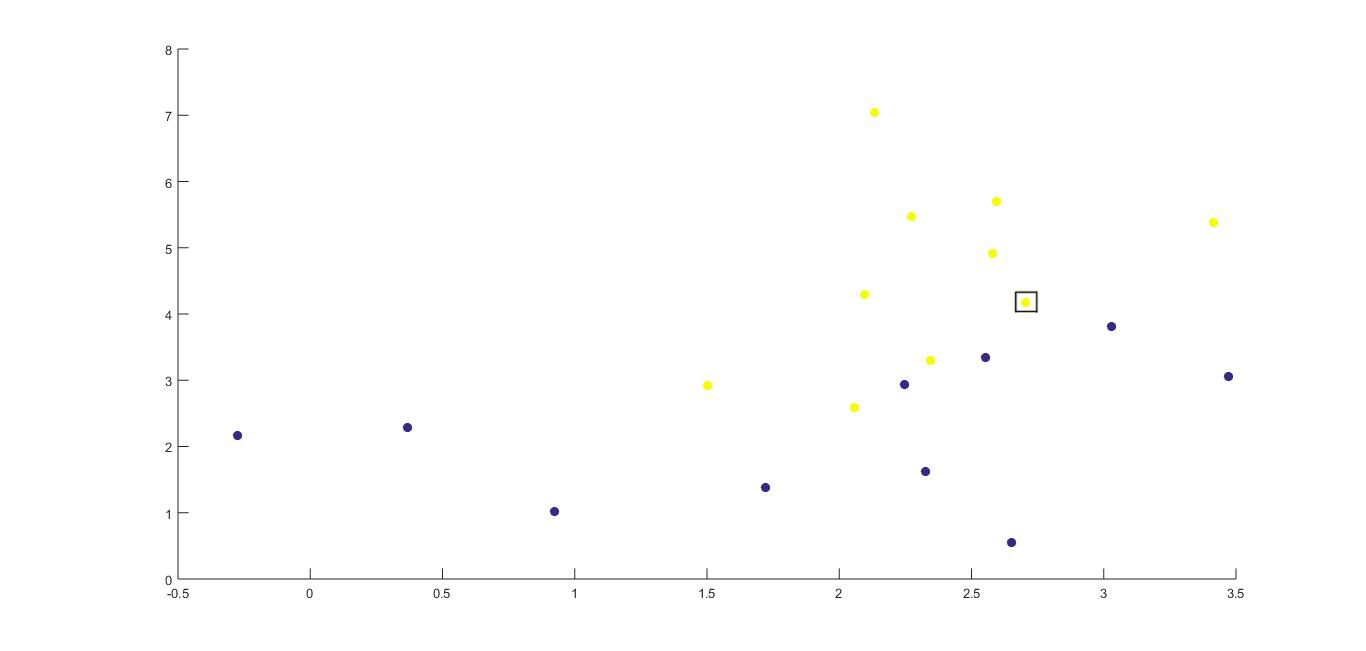
\includegraphics[width=1\textwidth]{fig1.jpg}
    \caption{example generated using matlab to demonstrate the average precision}
\end{figure}
The same computation will be done for all the samples in the space. and at the end we sum all the AP and divide them by the number of samples to obtain the mean average precision. As we can see the mean average precision put more weight on having the first result as a relevant sample(same class) than the second result and so on.
\subsection{The precision at k}
The precision at k is another ranking metric that is used to evaluate the result of a search query. As  its name indicates we are only interested of the precision at a given rank k. in our example we take the precision at 5 as a metric to evaluate the data. This metric is very useful to indicate if the user will get a relevant document in the 5 first result. A major disadvantage of this metric is that it does not take into consideration the position of that file in the result, meaning that, for a certain search query, if we have n out 5 relevant files it doesn't matter if the first one is relevant result or not. The precision at k is the average of all the precision of each sample alone.









\newpage
\begin{thebibliography}{2}
\bibitem{B00} 
Beth Logan
\textit{Mel Frequency Cepstral Coefficients for Music Modeling}. 
2000

\bibitem{AM11} 
J. Andén and S. Mallat. 
\textit{Multiscale scattering for audio classification.}. 
ISMIR 2011

\bibitem{A14} 
J. Andén 
\textit{Time and frequency scattering for audio classification}. 
January 7, 2014

\bibitem{H95}
Hermann Ludwig Ferdinand von Helmholtz
\textit{On the sensations of tone as a physiological basis}.
1895


\bibitem{P03}
Perfecto Herrera-Boyer and al.
\textit{Automatic Classification of Musical Instrument Sounds}.
Journal of New Music Research 2003


\bibitem{SOL}
Yan Maresz and al.
\textit{Ircam solo instruments UltimateSoundBank reference guide}

\bibitem{W09}
K. Q. Weinberger, L. K. Saul. 
\textit{Distance Metric Learning for Large Margin Nearest Neighbor Classification}.
Journal of Machine Learning Research (JMLR) 2009



\end{thebibliography}

\end{document}